\paragraph{Token Efficient Reinforcement Learning}
\label{sec:te}
Token efficiency is central to LLMs with test-time scaling. 
While test-time scaling inherently trades computation for reasoning quality, practical gains require algorithmic innovations that actively navigate this trade-off. 
Our previous findings indicate that imposing a problem-dependent budget effectively constrains inference-time compute, incentivizing the model to generate more concise chain of thought reasoning patterns without unnecessary token expansion \citep{team2025kimi,team2025kimik2}. 
However, we also observe a \emph{length-overfitting phenomenon}: models trained under rigid budget constraints often fail to generalize to higher compute scales. Consequently, they cannot effectively leverage additional inference-time tokens to solve complex problems, instead defaulting to truncated reasoning patterns.



To this end, we propose \emph{Toggle}, 
a training heuristic that alternates between {inference-time scaling} and {budget-constrained optimization}: 
for learning iteration $t$, 
the reward function is defined by 
\begin{align*}
\tilde{r}(x,y) = 
\begin{cases} 
r(x, y) \cdot \mathbb{I}\left\{ \frac{1}{K} \sum_{i=1}^K r(x, y_i)  < \lambda\ \mathrm{or}\ |y_i| \leq \mathrm{budget(x)} \right\} & \text{if } \lfloor t/m \rfloor \pmod 2 = 0\ (\mathrm{{Phase 0}}) \\
r(x, y) & \text{if } \lfloor t/m \rfloor \pmod 2 = 1\ (\mathrm{{Phase 1}}) 
\end{cases}
\, .
\end{align*}
where $\lambda$ and $m$ are hyper-parameters of the algorithm and $K$ is the number of rollouts per problem. 
Specifically, the algorithm alternates between two optimization phases every $m$ iterations:
\begin{itemize}

\item {Phase0} (\emph{budget limited phase}): 
The model is trained to solve the problem within a task-dependent token budget. 
To prevent a premature sacrifice of quality for efficiency, this constraint is conditionally applied: it is only enforced when the model's mean accuracy for a given problem exceeds the threshold $\lambda$.

\item {Phase1} (\emph{standard scaling phase}): The model generates responses up to the maximum token limit, encouraging the model to leverage computation for better inference-time scaling. 

\end{itemize}

The problem-dependent budget is estimated from the $\rho$-th percentile of token lengths among the subset of correct responses:
\begin{equation}
\mathrm{budget}(x) = \text{Percentile}\left(\{ |y_j| \mid r(x, y_i) = 1, i=1,\dots, K \}, \rho \right) \,.
\end{equation}
This budget is estimated once at the beginning of training and remains fixed thereafter. 
Notably, Toggle functions as a stochastic alternating optimization for a bi-objective problem. It is specifically designed to reconcile reasoning capabilities with computational efficiency. %In our experiments, we use $\lambda = 7/8$, $m=2$ and $\rho = 90\%$.


\begin{figure}[t]
    \centering
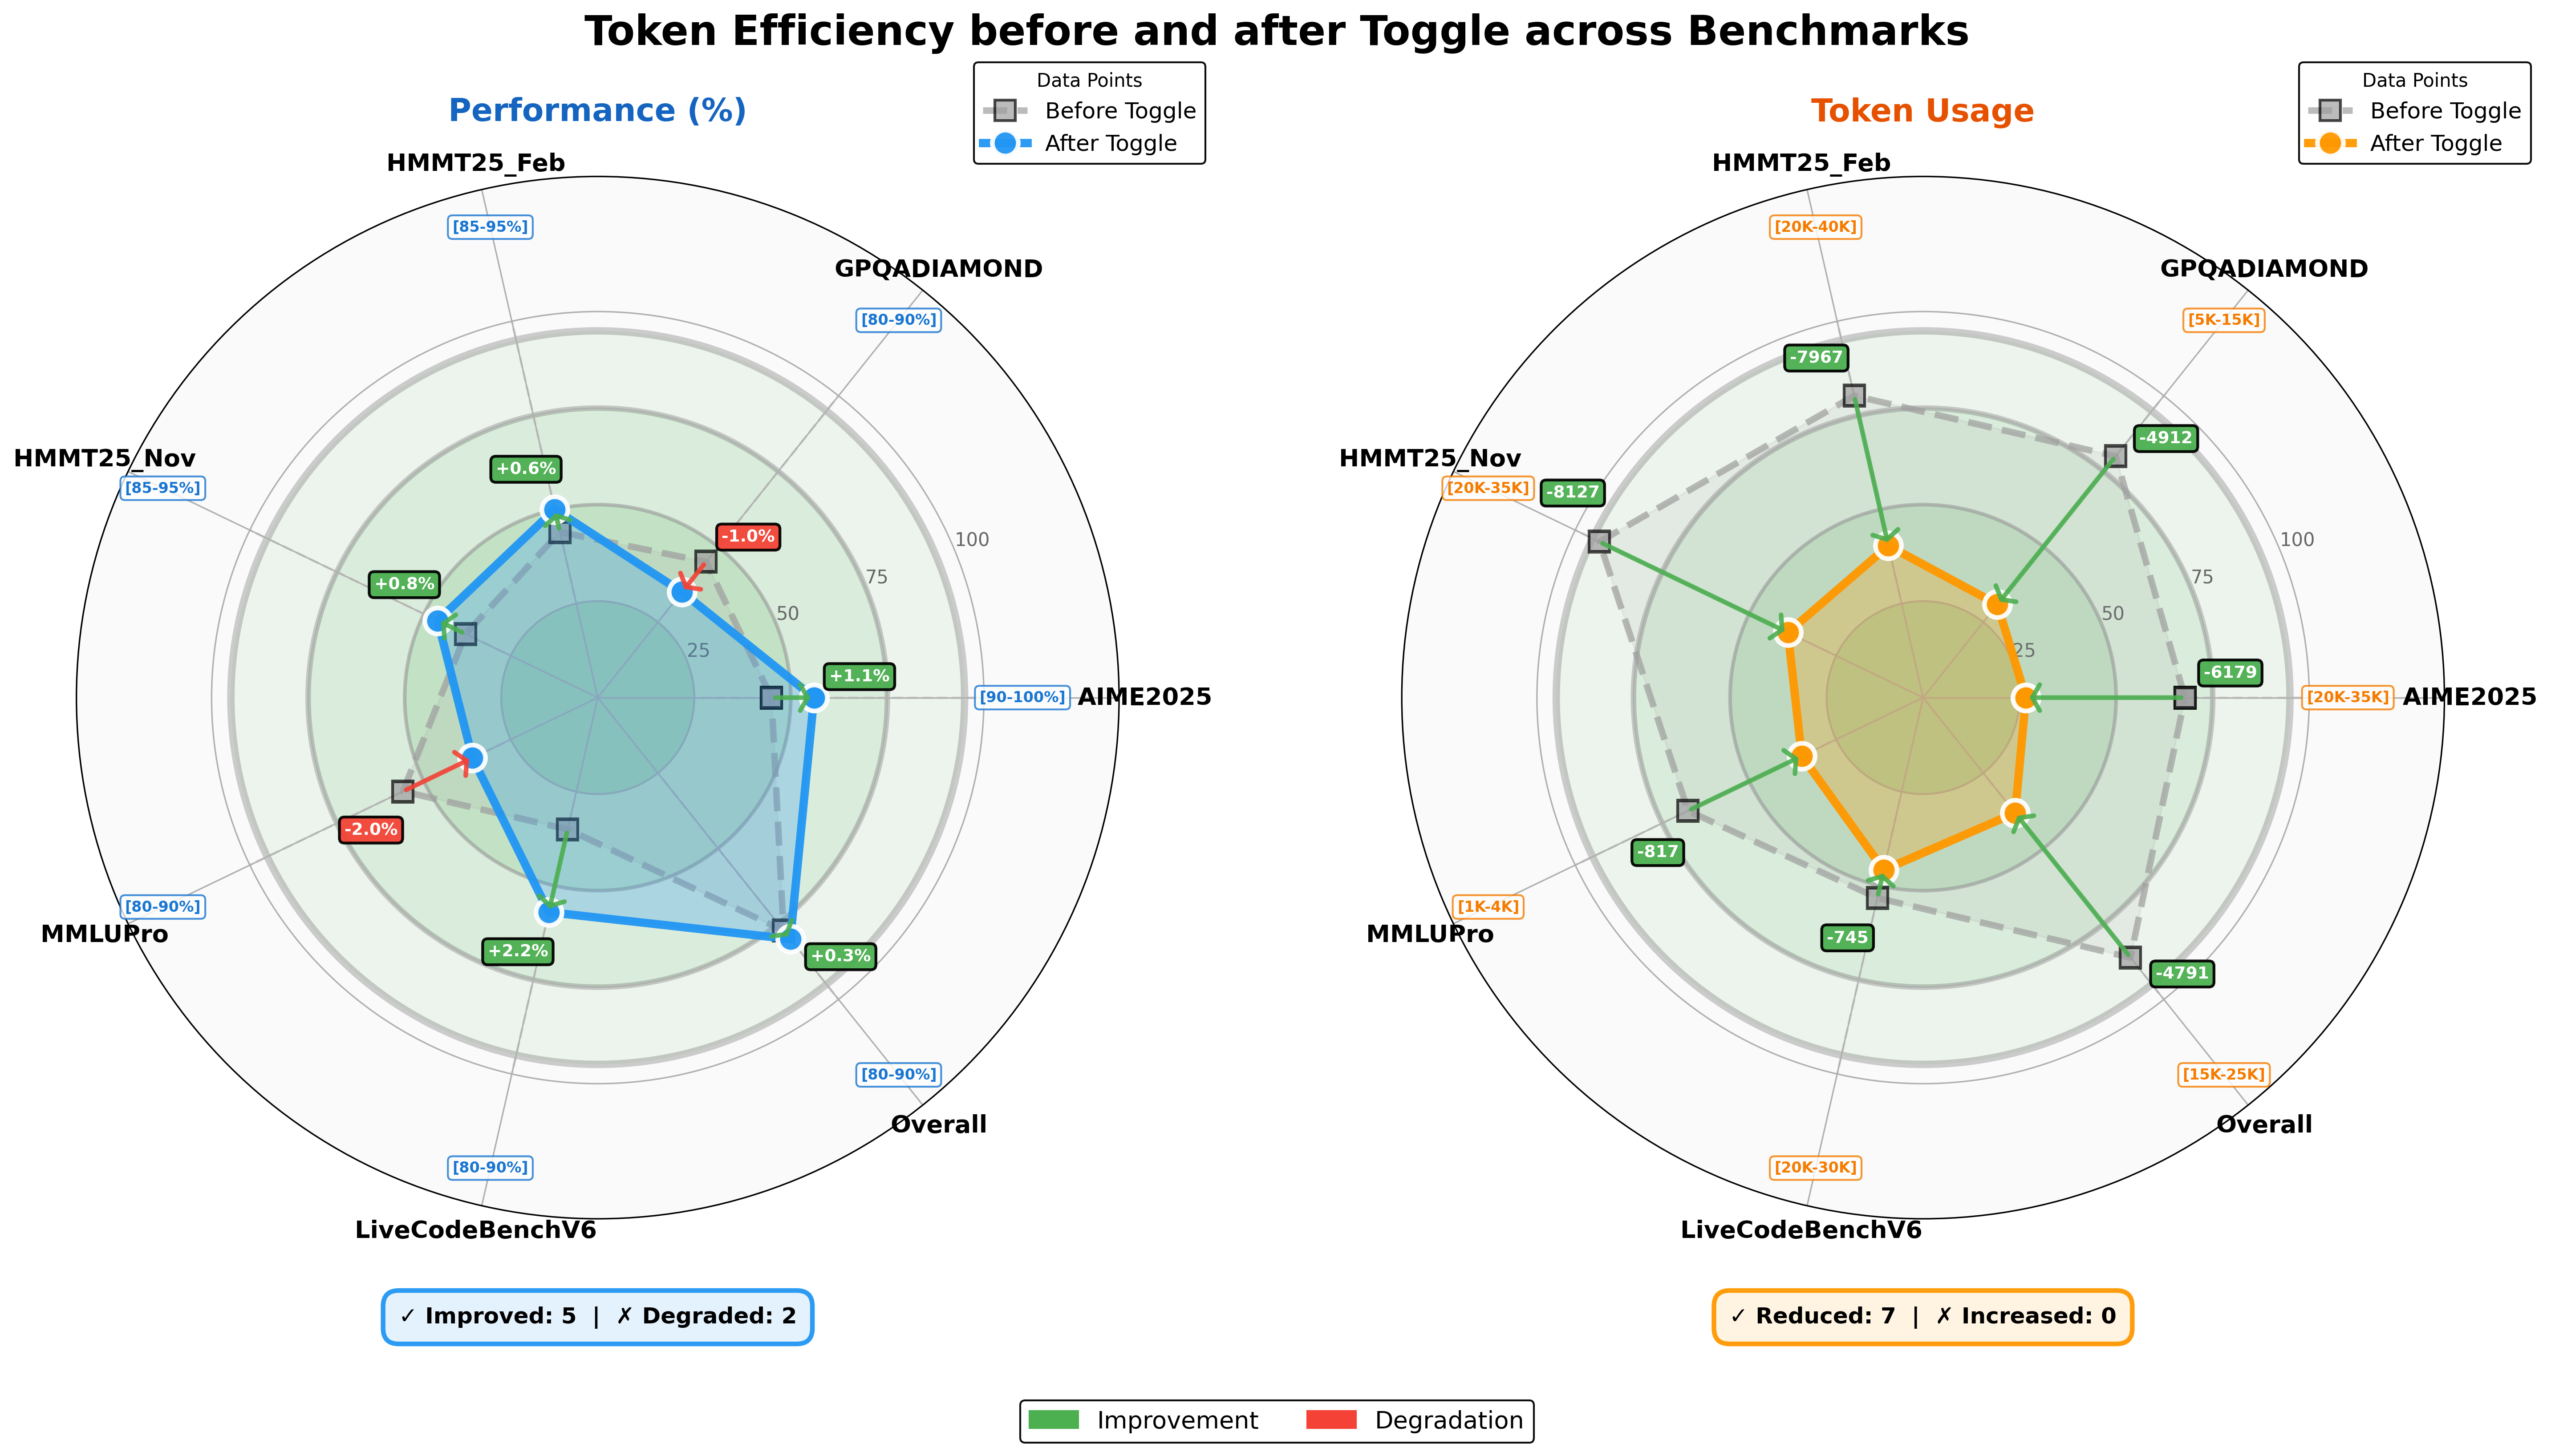
\includegraphics[width=0.8\linewidth, keepaspectratio]{figures/te-k2-thinking-radar.png}
    \caption{Comparison of model performance and token usage for Kimi K2 Thinking following token-efficient RL.}
    \label{fig:k25_performance}
\end{figure}

We evaluate the effectiveness of Toggle on K2 Thinking~\citep{moonshotai2025kimi}.
As shown in Figure~\ref{fig:k25_performance}, we observe a consistent reduction in output length across nearly all benchmarks.
On average, Toggle decreases output tokens by 25$\sim$30\% with a negligible impact on performance. 
We also observe that redundant patterns in the chain-of-thought, such as repeated verifications and mechanical calculations, decrease substantially.
Furthermore, Toggle shows strong domain generalization. 
For example, when trained exclusively on mathematics and programming tasks, the model still achieves consistent token reductions on GPQA and MMLU-Pro with only marginal degradation in performance (Figure \ref{fig:k25_performance}). 








